% -*- coding: utf-8; -*-

\chapter{Introduction}
Nowadays 3D surface models are used in several fields and industries such as medicine, engineering, entertainment, geo-exploration, architecture, cultural heritage and so on. These models can be acquired from a variety of sources like 3D scanning, 3D imaging, multi-view stereo reconstruction, CAD modeling, etc. The data generated by these techniques should be processed to be available for production or any task where it can be used (visualization, simulation, animation, interaction, etc.). This processing step is called digital geometry processing which is a field of computer science that uses mathematical models and algorithms \cite{BKPAL10}. Figure~\ref{fig:example} shows some examples of noisy meshes.



\begin{figure}
\centering
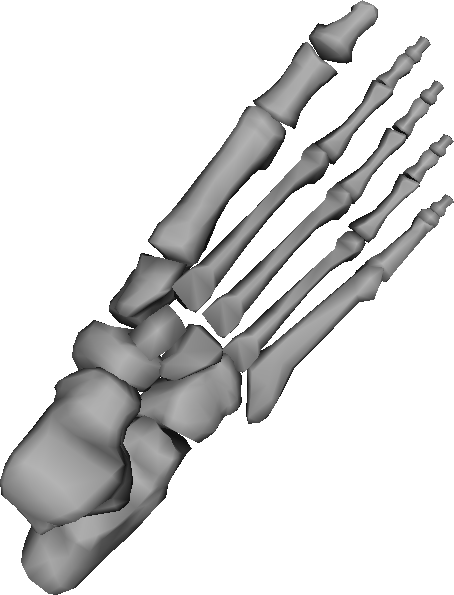
\includegraphics[width=0.45\textwidth]{pictures/image01.png}
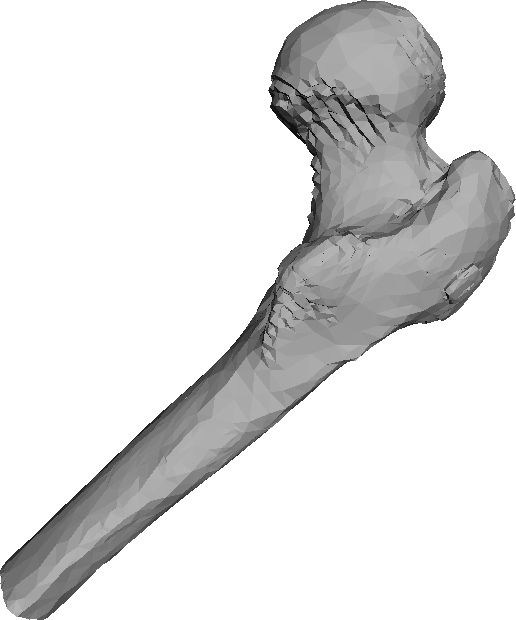
\includegraphics[width=0.45\textwidth]{pictures/image02.png}
\caption{Meshes generated from medical data. Data obtained from the AIM$@$SHAPE Shape Repository \cite{AIMSHAPE}}
\label{fig:example}
\end{figure}


This document is structured as follows. In Chapter~\ref{cha:Previous Work} we present some previous work relevant to our problem. In Chapter~\ref{cha:Proposal} we explain our proposal. In Chapter~\ref{cha:Results} we show our results. Finally, in Chapter~\ref{cha:Conclusion} we present our conclusion and future work.


